\documentclass[a4paper,10pt]{article}
\usepackage[utf8]{inputenc}
\usepackage{cite}
\usepackage[top=2.5cm,bottom=2.5cm,left=2.5cm,right=2.5cm]{geometry}
\usepackage[portuguese]{babel}
\usepackage{natbib}
\usepackage{graphicx}
\usepackage{url}

\title{Algoritmos de aproximação}
\author{Luiz Eduardo de Freitas Von Schmalz}
\date{abril, 2022}

\begin{document}

\maketitle
\begin{figure}[h!]
\centering
    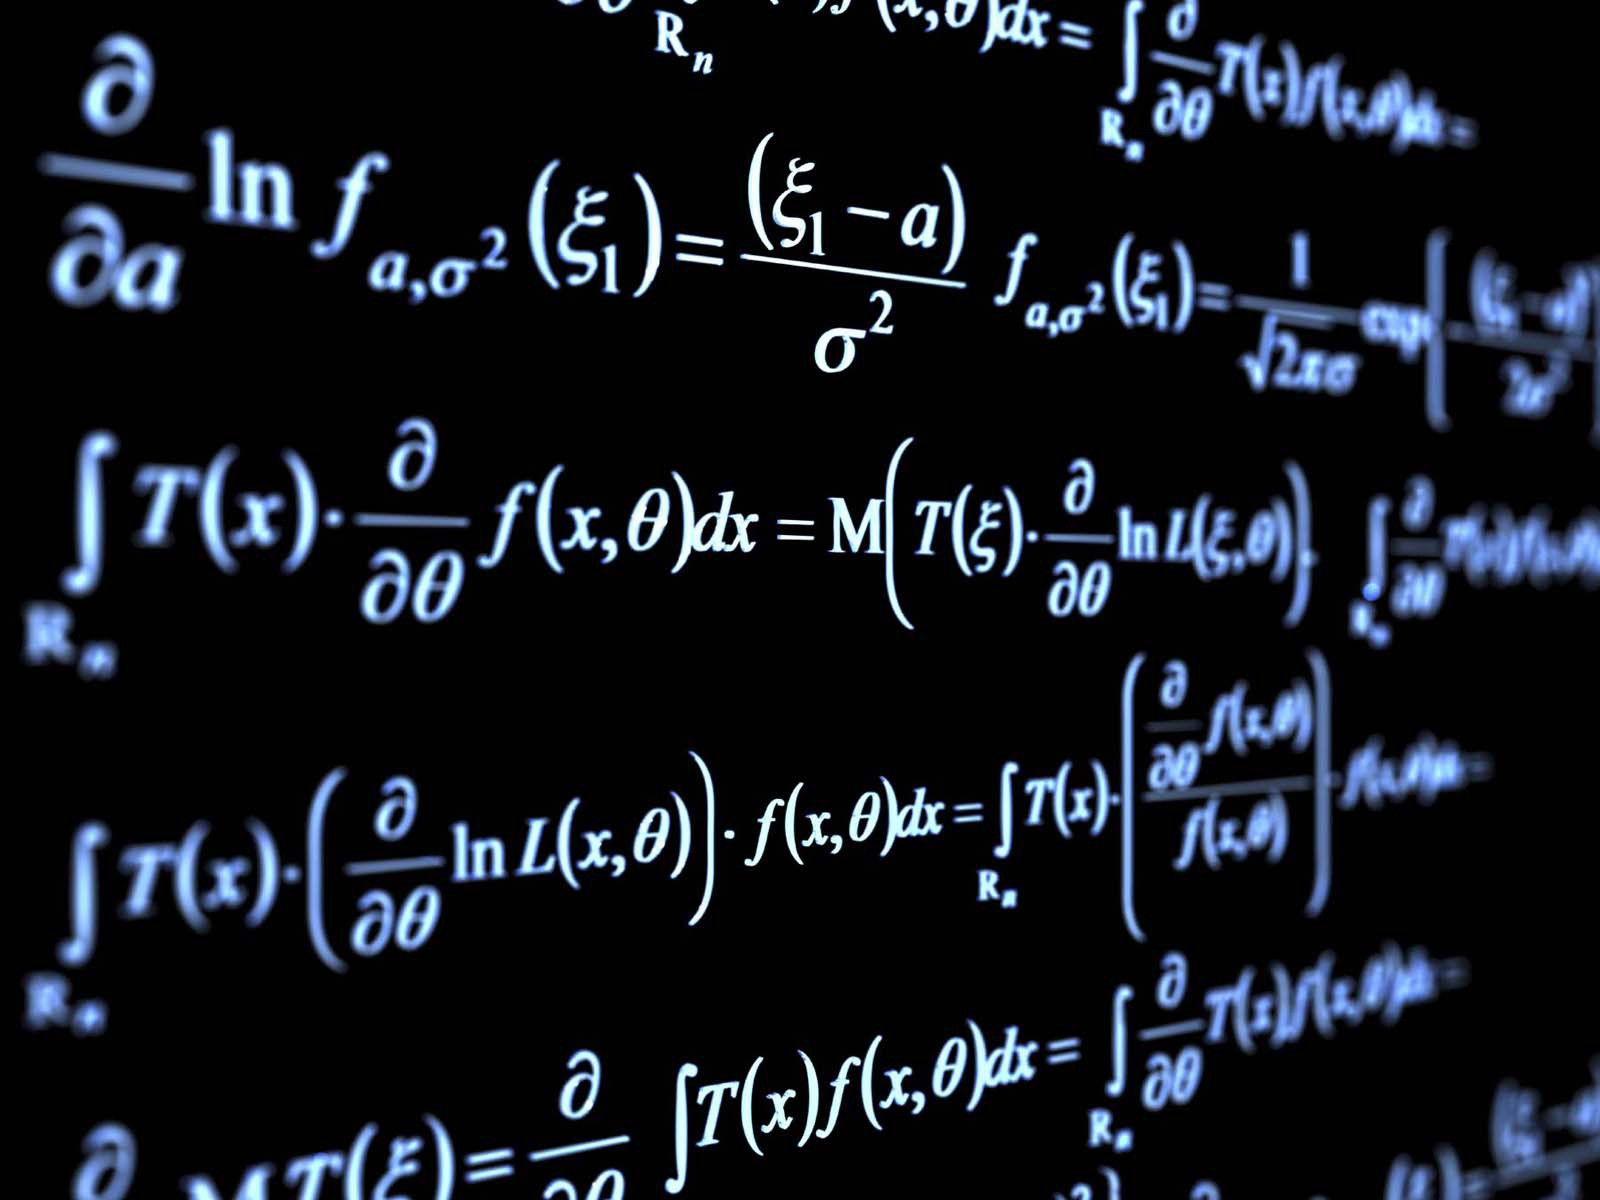
\includegraphics[width=100mm]{equacao3.jpg}
    \caption{Exemplo de equações grandes para as quais algoritmos de aproximação seriam muito úteis.}
\end{figure}
\section{Introdução}
\paragraph{}
    A disciplina IF766 - Algoritmos de aproximação é uma cadeira de extrema importância no curso de ciência da computação, ela se baseia na criação e compreensão de algoritmos para resolver problemas que sem os quais não seriam possíveis. Estamos falando de problemas que mesmo com algoritmos de aproximação demoraram muito tempo para serem resolvidos, estamos falando de meses ou até anos. \cite{algowiki}
    
\section{Relevância}
\paragraph{}
    Os problemas propostos são chamados de problemas de otimização, eles são geralmente associados a problemas NP-difíceis\cite{Npdificil}, que são problemas que não podem ser resolvidos em tempo polinomial, porém, também existem problemas que podem ser resolvidos em tempo polinomial mas seriam extremamente custosos em questão de tempo. Um exemplo clássico é o PTAS para o problema do caixeiro viajante euclidiano (PCV euclidiano, problema PCV utilizando distâncias euclidianas) concebido por Sanjeev Arora, que possui um tempo de execução de um ano. A princípio não parece vantajoso para a sociedade se prender tanto tempo a um único problema, porém, a aprendizagem de métodos pode ser de extremamente benéfico quando se trata de problemas reais que, a princípio, não tinham soluções, como problemas referentes à biologia computacional, engenharia financeira etc. 
    
\begin{figure}
\centering
    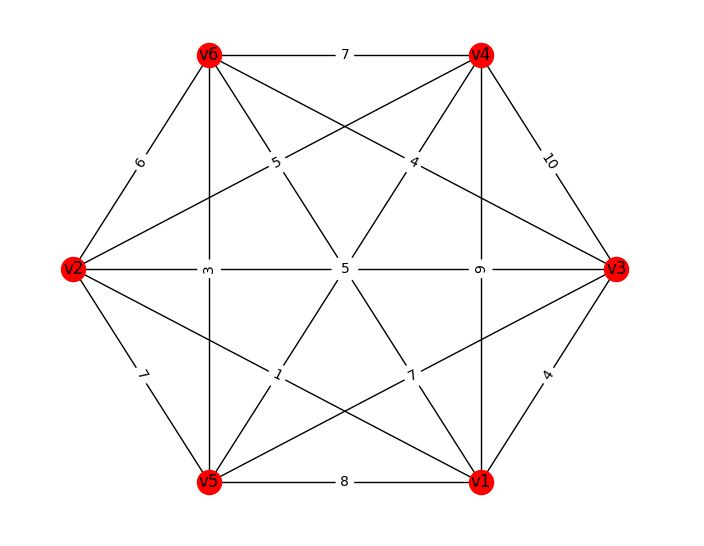
\includegraphics[width=130mm]{caixeiro.jpg}
    \caption{Ilustração do PCV euclidiano.}
    \cite{img}
\end{figure}
\paragraph{}

\section{Relação com outras cadeiras}

\paragraph{}
Em relação ao curso de ciência da computação, a disciplina de algoritmos de aproximação se encontra no sexto período e é uma cadeira eletiva, para ela não existem pré-requisitos e se resume em, de acordo com a ementa das disciplina),: ‘ABORDAGENS COMBINATÓRIAS; MÉTODO DE ARREDONDAMENTO; MÉTODO PRIMA-DUAL; CLASSES DE COMPLEXIDADE EM APROXIMAÇÃO.’. É uma cadeira que apesar de não ter pré-requisitos é cheia de conhecimentos avançados de matemática, então, é preciso um certo conhecimento desses tópicos antes de ingressar na mesma.

\bibliographystyle{plain}
\bibliography{ref.bib}
\end{document}

